\chapter{Experimental Evaluation}\label{chap:experimental_evaluation}
In this chapter we describe our approach to evaluate the performance of crowdsourced ontology validation steps. More precisely, in \hyperref[sec:evaluation_metrics]{Section~\ref*{sec:evaluation_metrics}} we start by describing all relevant performance metrics used to quantify the improvements. Then, in \hyperref[sec:evaluation_datasets]{Section~\ref*{sec:evaluation_datasets}} an overview of the used datasets~(e.g. ontologies) is given and finally, \hyperref[sec:crowdsourcing_task_interfaces]{Section~\ref*{sec:crowdsourcing_task_interfaces}} shows various interfaces which were presented to contributors to facilitate crowdsourcing task completion.

\subsubsection{Evaluation Hypothesis}
Based on existing efforts for ontology validation using crowdsourcing~(see \hyperref[sec:ucomp_protege_plugin]{Section~\ref*{sec:ucomp_protege_plugin}}), we formulate the following evaluation hypothesis:
\begin{quotation}
	The crowd performs ontology validation steps better if context is added to crowdsourcing tasks.
\end{quotation}

To evaluate the hypothesis stated above, we performed experimental evaluations on the implemented Protege~plugin. \hyperref[table:overview_exp_evaluation]{Table~\ref*{table:overview_exp_evaluation}} gives an overview of the experiments including their settings and used datasets, described thoroughly in the next sections. 
\begingroup
\renewcommand{\arraystretch}{1.5}
\begin{table}
	\begin{tabularx}{\textwidth}{l c *{4}{Y}}
		\toprule
		\multirow{2}{*}{\emph{Methods}} & \multicolumn{2}{c}{\emph{Data}} & \multicolumn{3}{c}{\emph{Crowdsourcing Settings}}\\
		\cmidrule(lr){2-3} \cmidrule(lr){4-6} 
		 & Ontology & No. of Classes & Judgements/ Price & Worker Selection & Quality Control\\
		\midrule
		 None, EC, NN, ES & Climate & 101 & $5/0.05$ & Level 3, AUS, UK, USA & Quiz\\
		 None, EC, NN, ES & Tennis & 52 & $5/0.05$ & Level 3, AUS, UK, USA & Quiz\\
		 None, EC, NN, ES & Finance & 77 & $5/0.05$ & Level 3, AUS, UK, USA & Quiz\\
		 \bottomrule
	\end{tabularx}
	\caption{Overview of performed ontology validation tasks, including datasets and settings.~~~~~~~\texttt{EC=Embedded Context, NN=Neighbouring Nodes, ES=External Source}}
	\label{table:overview_exp_evaluation}
\end{table}
\endgroup

%%%%%%%%%%%%%%%%%%%%%%%%%%%%%%%%%%%%%%%%%%%%%%%%%%%%%%%%%%%%%%%%%%%%%%%%%%%%%%%%%%%%%%%%%%%%%%%%%%%%%%%%%%%%%%%%%%%%%%%%%%%%%%%%%%%%%%%%%%%%%%%%%%%%

% SECTION: EVALUATION METRICS %
\section{Evaluation Metrics}\label{sec:evaluation_metrics}
To justify the improvements stated in the hypothesis, a detailed evaluation based on the metrics described below was performed. 

We used two approaches to measure the performance of the crowd. The first one requires some reference data which is compared against empirical data. This approach, originating from Information Retrieval~(IR), is called the \textbf{Golden~Standard~Approach}~\cite{brank2005}. To quantify the improvements/degradations, several metrics exist. On a binary classification scheme, as illustrated in \hyperref[fig:binary_classification_metrics]{Figure~\ref*{fig:binary_classification_metrics}}, these metrics are defined as fractions of \emph{True~Positives~(TP)}, \emph{True~Negatives~(TN)}, \emph{False~Positives~(FP)} and \emph{False~Negatives~(FN)}.
\begin{figure}
	 \centering
	 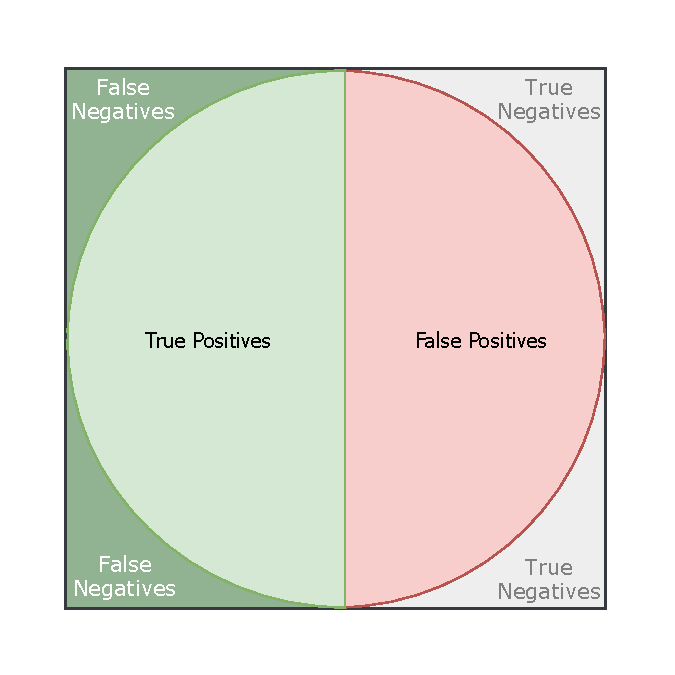
\includegraphics[width=0.5\textwidth]{drawio/Binary_Classification_Scheme}
	 \caption{Binary classification scheme for evaluation metrics of crowdsourcing tasks}\label{fig:binary_classification_metrics}
\end{figure}
In crowdsourcing contexts this means that yes-questions are either correctly~(TP) or incorrectly~(FN) answered and no-questions are either correctly answered~(TN) or incorrectly~(FP).

\paragraph{Precision} Precision is interpreted as the ratio of correctly answered yes-questions over the total number of answered yes-questions:
\[ Precision = \frac{TP}{TP + FP} \]
For concept relevance, values of Precision close to $1.0$ show that the crowd correctly rejects irrelevant concepts but maybe fails at accepting relevant ones. 
\paragraph{Recall} Recall is interpreted as the ratio of correctly answered yes-questions over the total number of available yes-questions:
\[ Recall = \frac{TP}{TP + FN} \]
For concept relevance, values of Recall close to $1.0$ show that the crowd correctly predicts relevant concepts but maybe fails at rejecting irrelevant ones. 

\paragraph{F-Measure} Unfortunately, exclusively relying on either of the above metrics has some drawbacks. For example, the crowd may correctly identify relevant concepts but fails at rejecting irrelevant ones~(high~Recall) or, on the other hand, irrelevant concepts may be correctly rejected whereas not all relevant ones may be detected~(high~Precision). 

The F-Measure compensates these flaws by combining Precision and Recall rates. The traditional F-Measure or balanced F-Score is calculated as the harmonic mean of Precision~(P) and Recall~(R):
\[ \mathit{F \mhyphen Measure} = 2 \cdot \frac{P \cdot R}{P + R} \]
In some situations researchers have criticised this metric that it may be biased~\cite{powers2011}. For this reason, there exists a modified version of the general F-Measure which takes an additional parameter $\beta$ into account:
\[ F_\beta = (1 + \beta^2) \cdot \frac{P \cdot R}{\beta^2 \cdot P + R} \]
Depending on the importance of Precision or Recall, $\beta$ can be set to a higher value~(e.g.~$F_2$), which weights Recall higher, or to a lower value~(e.g.~$F_{0.5}$), which puts more emphasis on Precision. Mostly, the generic F-Measure, also known as $F_1$ measure, is sufficient though, in which $\beta$ is set to $1$ to weight Precision and Recall evenly. 

The other approach in measuring the crowd's performance does not rely on reference values, instead, the metric reflects the agreement ratio among crowd workers. Therefore, the agreement ratio or \textbf{Inter-rater Agreement} measures, to what extend judges reached consensus. For binary tasks~(e.g. concept relevance checks), all possible outcomes are based on a table of 2x2~frequencies, as shown in \hyperref[fig:2x2_inter_rater_table]{Figure~\ref*{fig:2x2_inter_rater_table}}. In terms of evaluating concept relevance, this means that the crowd either agrees or disagrees whether a concept is relevant or not. 
\begin{figure}
	 \centering
	 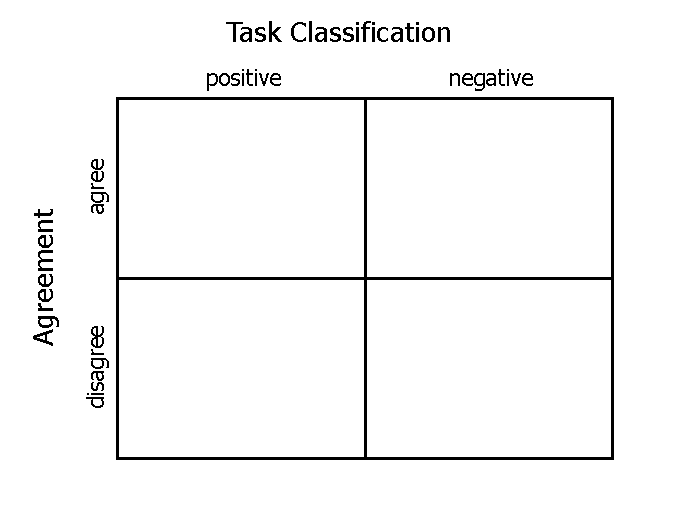
\includegraphics[width=0.5\textwidth]{drawio/Inter_Rater_Outcome_Table}
	 \caption{2x2 outcome table on Inter-rater Agreement for binary tasks}\label{fig:2x2_inter_rater_table}
\end{figure}

Several metrics exist to measure inter-rater reliability~\cite{zhao2013}. They primarily differ in to what extent judgements made by chance are taken into account. In our evaluation though, the following metric is used:
\paragraph{Percentage Agreement}
This is the simplest and most commonly used metric, which is calculated by dividing the number of agreeing raters~($A$) by the total rater count~($N$).
\[ Agreement = \frac{A}{N} \]
Despite its intuitive appeal, it has been criticised, that it does not take the agreements made by chance into account~\cite{hunt1986}. On the other hand, calculation of chance-adjusted metrics is more complex and have the potential to over- or undervalue the corrections for chance.  
Moreover, reliability is assumed to be very high because crowdsourcing settings were adjusted to sort out random answers. A more detailed discussion on this topic is given, when the evaluation setup is described.  


% SECTION: DATASETS %
\section{Datasets}\label{sec:evaluation_datasets}
Within the next paragraphs, ontologies used as the input for evaluation tasks are described in more detail. As this thesis builds upon existing work~\cite{wohlgenannt2016}, it makes sense to use the same ontologies as evaluation source. Also, we had access to the raw evaluation data which they had used in their experiments. 

The main characteristics of the three ontologies used for evaluation are summarised in \hyperref[table:dataset_ontologies]{Table~\ref*{table:dataset_ontologies}}. 
\begingroup
\renewcommand{\arraystretch}{1.5}
\begin{table}
	\begin{tabularx}{\textwidth}{l c *{3}{Y}}
		\toprule
		\multirow{2}{*}{\emph{Number of}} & \multicolumn{3}{c}{\emph{Ontology}}\\
		\cmidrule(l){2-4} 
		  & Climate Change & Tennis & Finance \\
		\midrule
		 Classes  & 101 & 52 & 77 \\
		 Properties  & 28 & 34 &  29 \\
		 SubClass Relations  & 84 & 35 & 78 \\
		 Individuals  & 64 & 33 & 47 \\
		\bottomrule
	\end{tabularx}
	\caption{Characteristics of the used ontologies}
	\label{table:dataset_ontologies}
\end{table}
\endgroup
Two of these ontologies, covering the domains \emph{climate change} and \emph{tennis}, emerged from seed ontologies used in an ontology learning algorithm~\cite{liu2005semi}. They evolved from several rounds of adding more input data~\cite{wohlgenannt2012}. The other ontology covers the finance domain and represents a small subset of the vocabulary defined by the Multilingual Thesaurus of the European Union~(EuroVoc)\footnote{\url{http://eurovoc.europa.eu/drupal/?q=evontology} accessed 2018/07/13}.

The tested ontologies are of limited size which makes evaluation easier, but still has significance for testing the impact of context enrichment in ontology validation. Whereas the \emph{Climate Change} ontology contains 101 concepts, 28 object properties, 64 individuals and 84 subclass relations, the \emph{Finance} ontology is of smaller size, containing 77 concepts, 29 object properties, 47 individuals and 78 subclass relations. The \emph{Tennis} ontology has 119 entities in total, 52 of which are concepts, 34 object properties and 33 individuals. 

\subsubsection{Evaluation Setup}
For calculating evaluation metrics the ontologies need to be annotated with reference values. From previous experiments~\cite{wohlgenannt2016} evaluation data was consolidated and annotations were generated. Unfortunately, for some concepts we had ambiguous data or none at all. We manually verified the enriched ontologies by excluding incorrect annotations and adding missing ones where appropriate. This was an important task, particularly because learned ontologies often contain inconsistent and inaccurate data. 

Concerning crowdsourcing tasks, Figure Eight\footnote{\url{https://www.figure-eight.com/} accessed 2018/07/16}~(former CrowdFlower) allows adjusting a variety of settings. We paid $\$0.05$ per task, required 5 judgements per unit and restricted judgements to the highest quality level of crowd workers~(Level 3). Additionally, we made the assumption that all labels of the validated ontologies are in English, therefore achieving results of higher quality requires restricting participation to the following English speaking countries: Australia, United Kingdom and United States. Furthermore, crowd workers had to correctly answer 8~quiz~questions from politics, computing and tennis. Although this does not prevent contributors from randomly answering test questions, it provides at least a minimum of quality control. Without any quality control measures, results would be of little use, as a recent survey reveals~\cite{daniel2018}. 

A central part of the assessment is the definition of evaluation tasks. Crowd workers were consulted to assist in the following ontology engineering task: \textbf{Verification of Domain Relevance}. For each concept selected for evaluation crowd workers need to decide whether it is relevant for the domain in question~(in our case, Climate Change, Tennis and Finance).
Using domain relevance, we evaluated our proposed methods of context enrichment
\emph{Ontology~based~Approach}~(\hyperref[sec:enrichment_ontology_approach]{Section~\ref*{sec:enrichment_ontology_approach}}),
\emph{Metadata~based~Approach}~(\hyperref[sec:enrichment_metaData_approach]{Section~\ref*{sec:enrichment_metaData_approach}}) and
\emph{Dictionary~based~Approach}~(\hyperref[sec:enrichment_dictionary_approach]{Section~\ref*{sec:enrichment_dictionary_approach}}).
Each of which generates textual descriptions which were added to the crowdsourcing task. For the Embedded Context Approach we had to manually annotate the ontologies with descriptions using the Dublin~Code~Metadata~Set~(e.g. \texttt{dc:description}). For the External Source Approach the WordNik~API\footnote{\url{https://developer.wordnik.com/} accessed 2018/06/15} was consulted to provide example sentences for requested concepts. 



% SECTION: CROWDSOURCING TASK INTERFACES %
\section{Crowdsourcing Task Interfaces}\label{sec:crowdsourcing_task_interfaces}



%%%%%%%%%%%%%%%%%%%%%%%%%%%%%%%%%%%%%%%%%%%%%%%%%%%%%%%%%%%%%%%%%%%%%%%%%%%%%%%%%%%%%%%%%%%%%%%%%%%%%%%%%%%%%%%%%%%%%%%%%%%%%%%%%%%%%%%%%%%%%%%%%%%%
